\chapter{Results and Discussion}
\label{chap:results}

In the following, we present benchmarks for the ballot validity proofs in our voting schemes.
Additionally, we present separate benchmarks for proving choice space membership and proving correct encryption.
Here, we use SageMath to generate the inputs for the ballot validity circuits, Circom to implement the circuits and snarkjs to conduct the actual proofs (\cref{chap:software}) in a Groth16 \gls{zps}.

For every benchmarked circuit, we record the constraint count , $CRS$ size and $CRS$ generation time\footnote{
    \label{footnote:crsBasedOnPtauFile}
    Here, we create $CRS$ based on the same pregenerated file \UseVerb{ptau} for every circuit (\cref{section:software:snarkjsSetup}).
},
proving time and verification time\footnote{
    \label{footnote:ignoreProofVerificationTimes}
    To verify a \gls{zkp} over a circuit, we use \cref{alg:verifyG16}.
    Here, the only computation that depends on the circuit is
    \begin{align*}
        g_1^I\gets \left(\textcolor{cyan}{g_1^\frac{\beta A_0(\tau)+\alpha B_0(\tau)+C_0(\tau)}{\gamma}}\right)\odot_{\mathbb{G}_1}\prod\limits_{j=1}^{n_I}\left(\textcolor{cyan}{g_1^\frac{\beta A_{p^{-1}(j)}(\tau)+\alpha B_{p^{-1}(j)}(\tau) + C_{p^{-1}(j)}(\tau)}{\delta}}\right)^{I_j}\text{.}
    \end{align*}
    However, compared to the computations needed for the proving algorithm, this is negligible.
    In practice, verification times for all benchmarked cases remain under $1.5$ seconds.
    Therefore, we do not compare the verification times in more detail.
}.

We compare our findings to the results obtained by Huber et. al. using libsnark \cite{huber_zk-snarks_2025}.\footnote{
    \label{footnote:noCompForCRSGenerationTimes}
    Note that Huber et. al. did not record $CRS$ generation times.
    Therefore, we cannot compare this metric.
    However, in practical applications of voting schemes, the $CRS$ for $\mathfrak{C}_{C}^{Ballot\text{-}Validity}$ would likely be included in the voting software or be publicly accessible.
    Specifically, such a software would either include multiple $CRS$ for some selected election types with specified parameters or publish this information to their \gls{pbb}.
    Then, the $CRS$ generation times are irrelevant.
}

As in the work of Huber et. al., all our benchmarks were conducted on an ESPRIMO Q957 ($64$-bit, i5-7500T CPU @ 2.70GHz, $16$GB RAM).
We observed that the $CRS$ generation phase and the $16$GB of RAM are the main limiting factor.
This allows us to compute \glspl{g16snark} over circuits with roughly $6$ million times at most.
Therefore, computing and verifying \glspl{g16snark} over a circuit with an even higher constraint count could be possible on our test system if the $CRS$ for this circuit is provided.
However, even with a $6$ million constraint limit, proving times reach $400$s and $CRS$ sizes reach $3.6$GB which is at the limit for most practical applications of voting schemes. \todo{Is it? Find reference.}

\section{Asserting Encryption via $\mathfrak{C}_C^{Enc}$}
\label{section:results:assertEncryption}
The circuit $\mathfrak{C}_C^{Enc}$ is used to assert the a ballot $b$ corresponds to an encrypted ballot $b'$ where both $b$ and $b'$ are provided as inputs to the circuit (\cref{section:ourVotingSchemes:ballotValidity}).

In their approach, Huber et. al. use an \gls{eeg} encryption scheme based on the Montgomery curve $M_{126932, 1}(\mathbb{F}_qP^2)$ to implement $\mathfrak{C}_{C}^{Enc}$ in libsanrk \cite{huber_zk-snarks_2025}.
We implement the same option in Circom (\cref{fig:circuit:encMEEG}).
Additionally, we implement $\mathfrak{C}_{C}^{Enc}$ using a \gls{ppeeg} encryption scheme based on the Twisted Edwards curve $TE_{126934, 126930}(\mathbb{F}_q)$ isomorphic to $M_{126932, 1}(\mathbb{F}_qP^2)$ (\cref{fig:circuit:encTEPPEEG}).

Since ballots are encrypted componentwise, we benchmark the circuit $\mathfrak{C}_C^{Enc}$ for ballots with different numbers of entries.
Moreover, the size of the circuit $\mathfrak{C}_C^{Enc}$ depends on the number of bits which we use to represent individual ballot entries.

The results of our benchmarks and the comparison with the results obtained by Huber et. al. \cref{fig:plots:Circom_libsnark_Enc}.
Note that we compare results for encrypting ballot entries represented with $1$, $16$ and $32$ bits since those are the cases also covered by Huber et. al. \cite{huber_zk-snarks_2025}.\footnote{
    \label{footnote:bitPracticalityEnc}
    Using more than $32$ Bits to represent a ballot entry $v$ is infeasible in practice as decryption requires finding $v$ based on $g^v$.
    This is hard according to the Discrete Logarithm problem if $v$ can assume a lot of different values.
}
However, we also tested our implementation with up to $250$ bits per ballot entry as shown in \cref{todo}.\footnote{
    \label{footnote:bitLimitEnc}
    Note that using more than $250$ bits to represent ballots is not possible in our voting schemes.
    We use group with order 
    \begin{align*}
        p=2736030358979909402780800718157159386074658810754251464600343418943805806723
    \end{align*}
    as the basis for our \gls{eeg} or \gls{ppeeg} encrpytion scheme.
    Here, $p$ is a $251$-Bit number. 
    Since we use $g^{v}$ for a generator $g$ to represent a ballot entry $v$ in those encryption schemes, we can use at most $250$ Bits to represent $v$ unambiguosly.
    %
    %However, even using more than $32$ Bits to represent a ballot entry $v$ is infeasible in practice as decryption requires finding $v$ based on $g^v$.
    %This is hard according to the Discrete Logarithm problem if $v$ can assume a lot of different values.
}\todo{Make in Appendix}


% In addition to that, we compare our results to those obtained by Huber et. al. as shown in \cref{fig:plots:Circom_libsnark_Enc}.\footnote{
%     \label{footnote:encBitLimitationLibsnark}
%     Note that we only compare results for encrypting ballot entries represented with $1$, $16$ and $32$ bits since those are the cases also covered by Huber et. al. \cite{huber_zk-snarks_2025}.
% }

% \begin{figure}[h]
%     \centering
%     \begin{subfigure}{\textwidth}
%         \centering
%         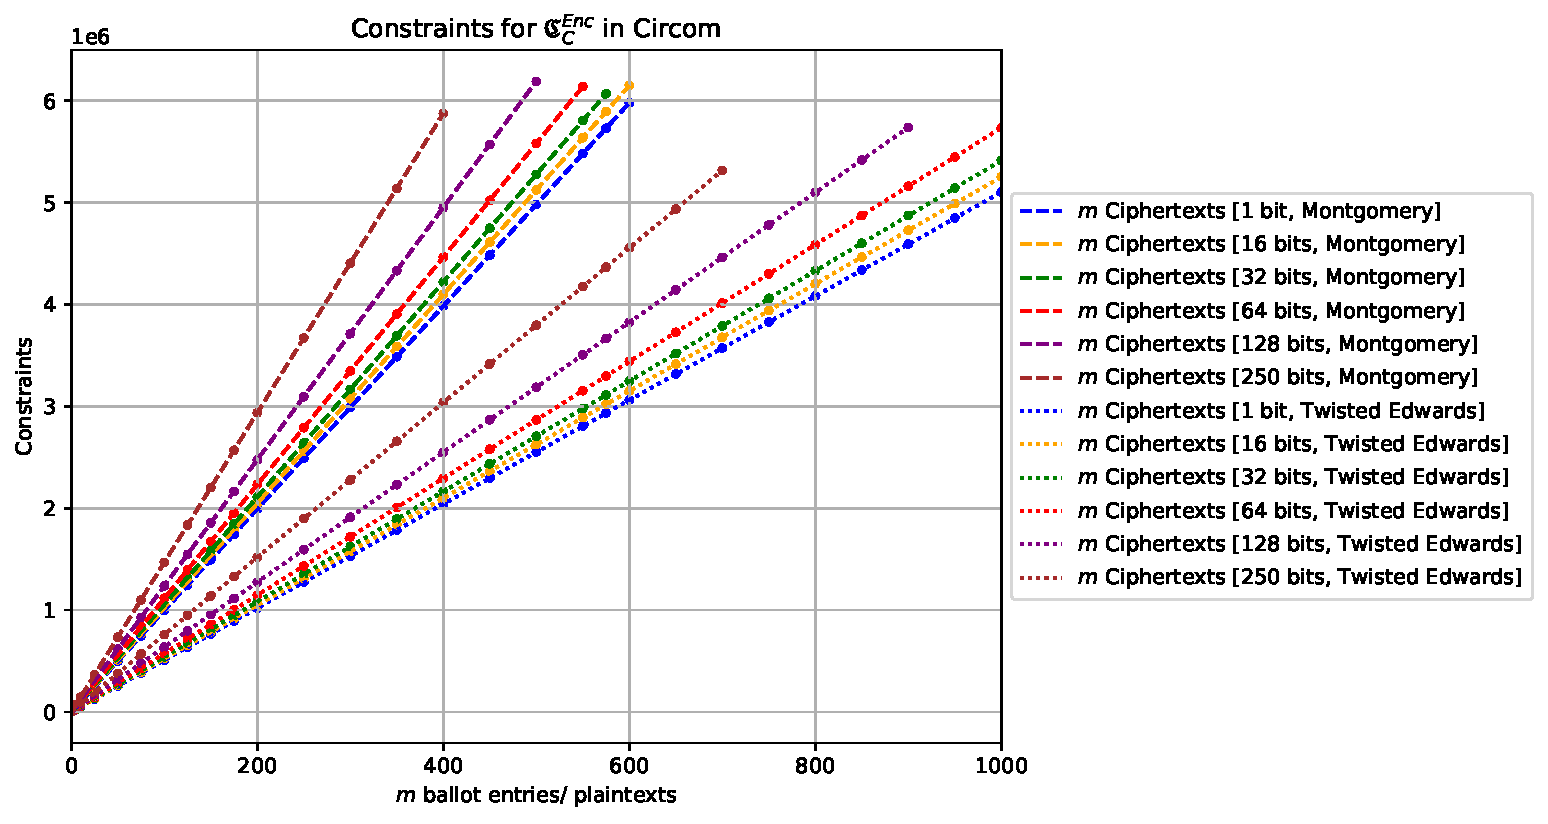
\includegraphics[scale=.6]{../src/benchmarks/plotting/plots/encryption/MontgomeryTwistedEdwards/EncryptionMontgomeryTwistedEdwardsConstraints.pdf}
%         \caption{Number of constraints.}
%         \label{fig:plots:M_TE_Enc_Constraints}
%     \end{subfigure}
%     \\
%     \begin{subfigure}{\textwidth}
%         \centering
%         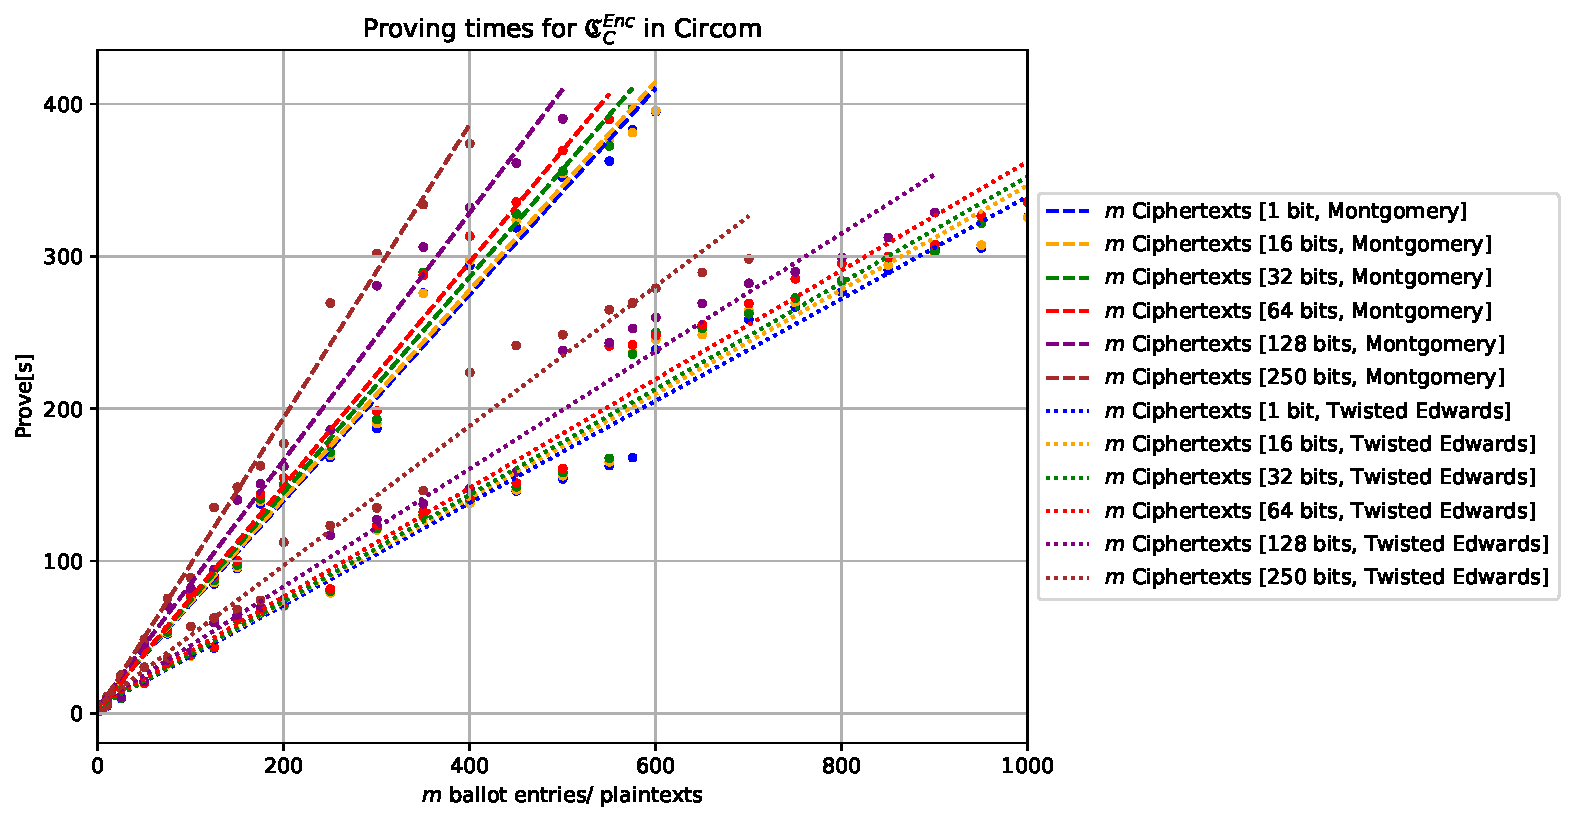
\includegraphics[scale=.6]{../src/benchmarks/plotting/plots/encryption/MontgomeryTwistedEdwards/EncryptionMontgomeryTwistedEdwardsProve[s].pdf}
%         \caption{Proving time.}
%         \label{fig:plots:M_TE_Enc_Prove}
%     \end{subfigure}
% \end{figure}%
% \begin{figure}[h]\ContinuedFloat
%     \centering
%     \begin{subfigure}{\textwidth}
%         \centering
%         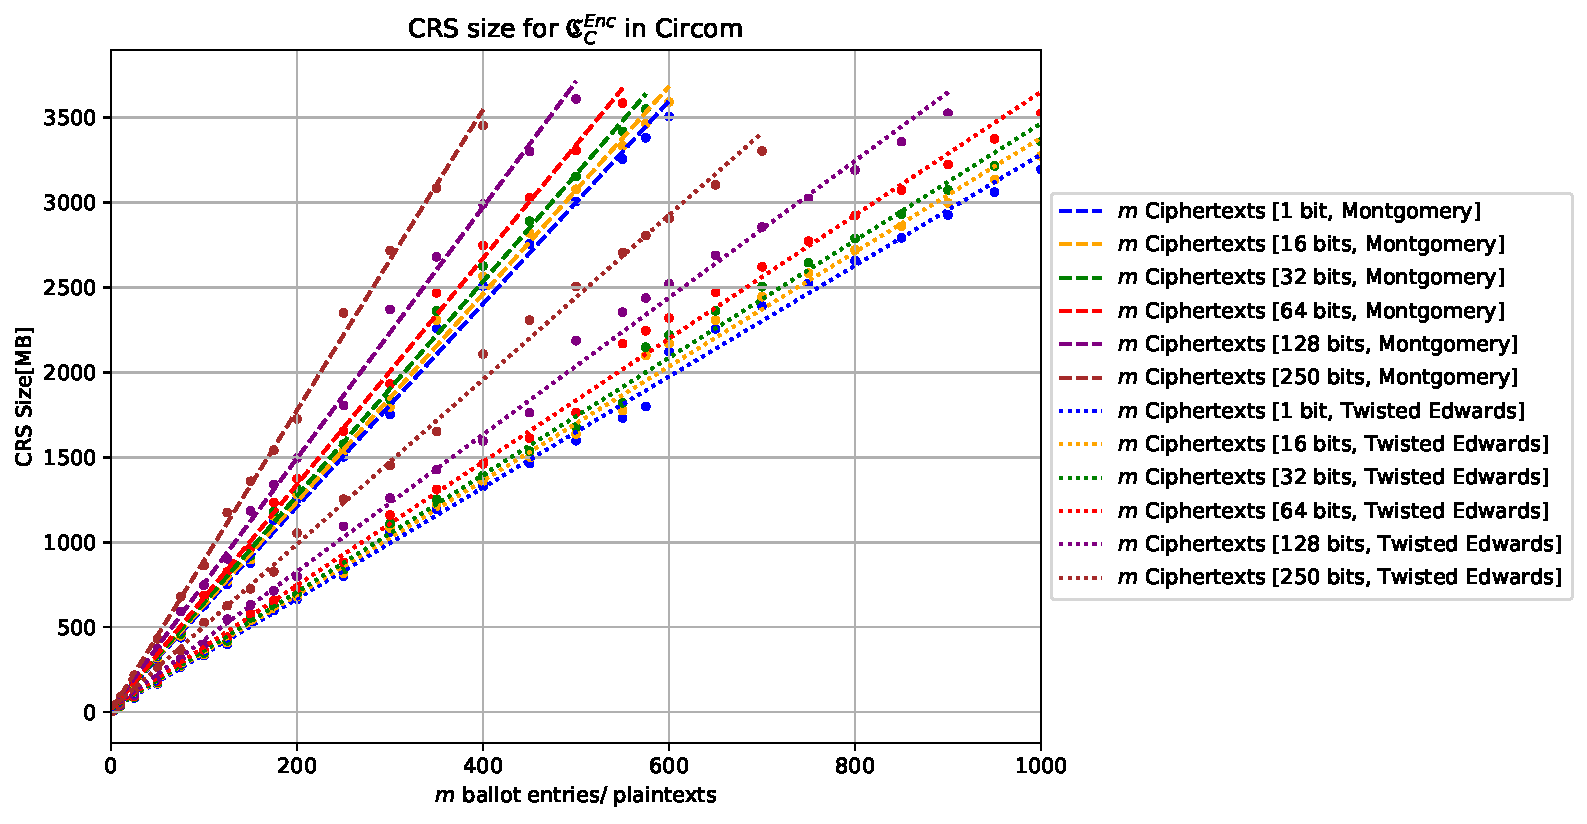
\includegraphics[scale=.6]{../src/benchmarks/plotting/plots/encryption/MontgomeryTwistedEdwards/EncryptionMontgomeryTwistedEdwardsCRS Size[MB].pdf}
%         \caption{Size of the $CRS$.}
%         \label{fig:plots:M_TE_Enc_CRSSize}
%     \end{subfigure}
%     \\
%     \begin{subfigure}{\textwidth}
%         \centering
%         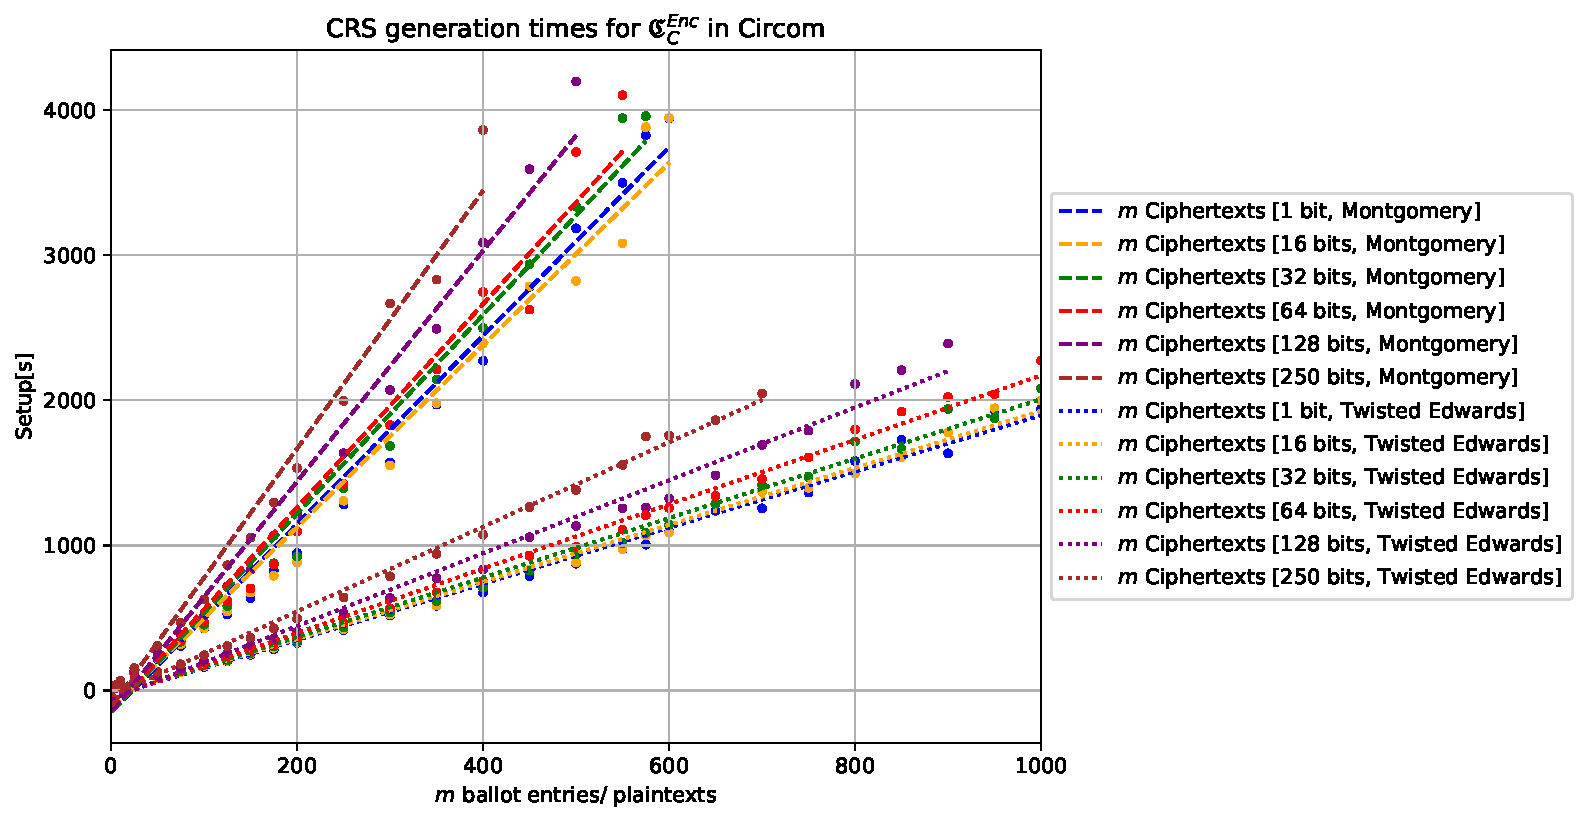
\includegraphics[scale=.6]{../src/benchmarks/plotting/plots/encryption/MontgomeryTwistedEdwards/EncryptionMontgomeryTwistedEdwardsSetup[s].pdf}
%         \caption{Time needed to generate the $CRS$ from an existing \UseVerb{ptau} file.}
%         \label{fig:plots:M_TE_Enc_Setup}
%     \end{subfigure}
%     \caption{Number of constraints, proving times, $CRS$ sizes and $CRS$ generation times needed for the \gls{g16snark} over for $\mathfrak{C}_{C}^{Enc}$ in Circom using Montgomery and Twisted Edwards curves.}
%     \label{fig:plots:M_TE_Enc}
% \end{figure}

\begin{figure}[h]
    \centering
    \begin{subfigure}{\textwidth}
        \centering
        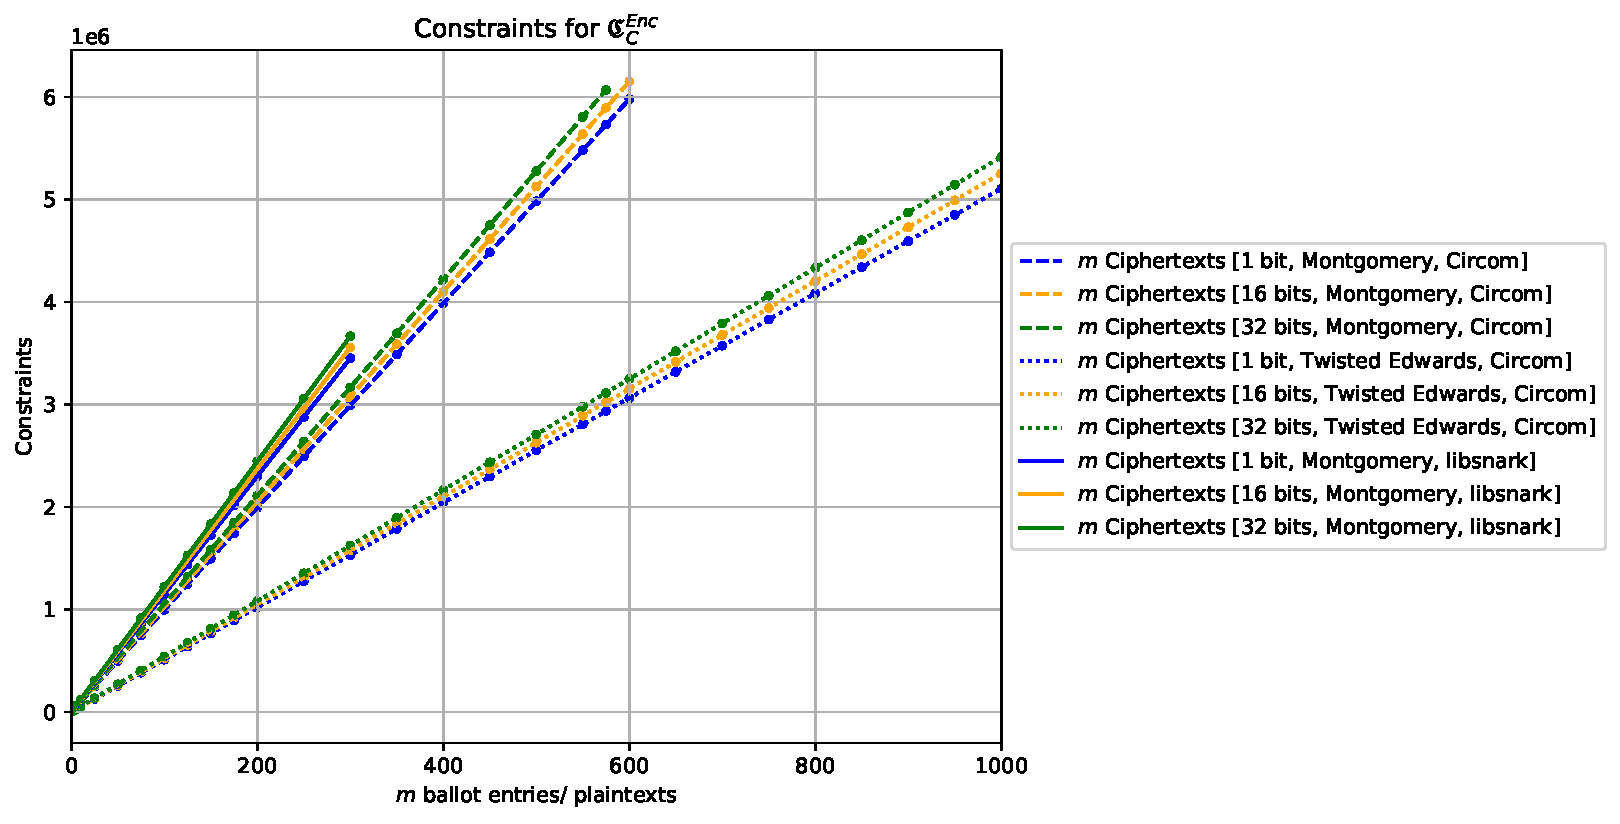
\includegraphics[scale=.6]{../src/benchmarks/plotting/plots/encryption/Comparison/EncryptionComparisonConstraints.pdf}
        \caption{Number of constraints.}
        \label{fig:plots:Circom_libsnark_Enc_Constraints}
    \end{subfigure}
    \\
    \begin{subfigure}{\textwidth}
        \centering
        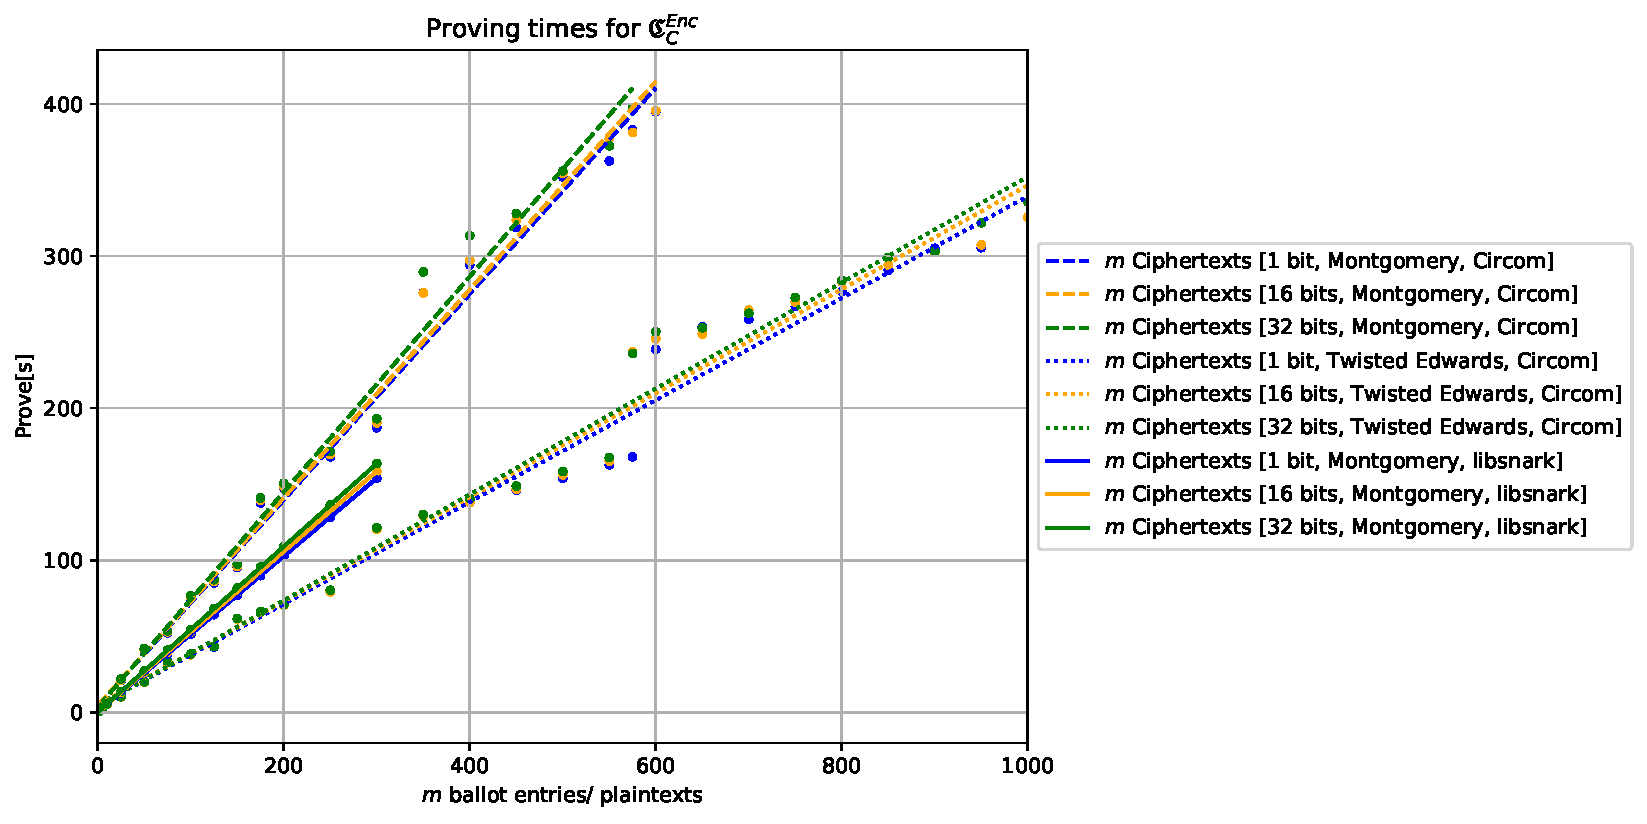
\includegraphics[scale=.6]{../src/benchmarks/plotting/plots/encryption/Comparison/EncryptionComparisonProve[s].pdf}
        \caption{Proving time.}
        \label{fig:plots:Circom_libsnark_Enc_Prove}
    \end{subfigure}
\end{figure}

\begin{figure}[h]\ContinuedFloat
    \centering
    \begin{subfigure}{\textwidth}
        \centering
        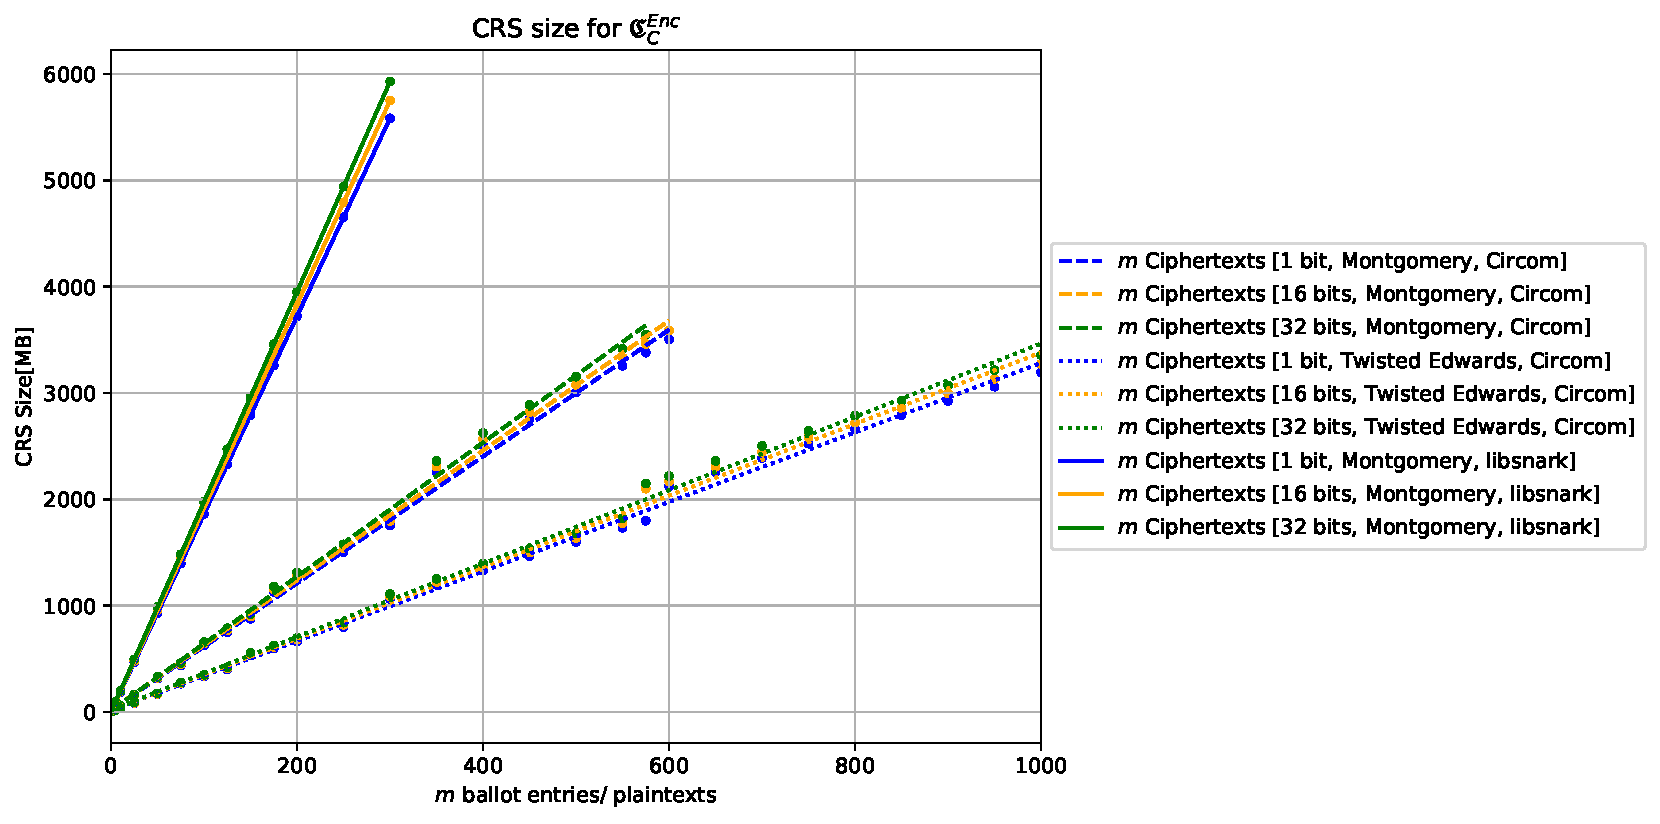
\includegraphics[scale=.6]{../src/benchmarks/plotting/plots/encryption/Comparison/EncryptionComparisonCRS Size[MB].pdf}
        \caption{Size of the $CRS$.}
        \label{fig:plots:Circom_libsnark_Enc_CRSSize}
    \end{subfigure}
    \caption{Number of constraints, proving times and $CRS$ sizes needed for the \gls{g16snark} over for $\mathfrak{C}_{C}^{Enc}$ using Montgomery and Twisted Edwards curves in Circom and using Montgomery curves in libsnark.\cref{footnote:noCompForCRSGenerationTimes}}
    \label{fig:plots:Circom_libsnark_Enc}
\end{figure}

\todo{Discussion}

\section{Asserting Choice space membership via $\mathfrak{C}_C^{Vot}$}
\label{section:results:asertVoting}
The circuit $\mathbb{C}_C^{Vot}$ is used to assert that a ballot $b$ is part of the choice space $C$ (\cref{section:ourVotingSchemes:ballotValidity}).
Here, the ballot $b$ and depending on the election type also a ranking $r=aux^{Vot}$ are provided as inputs to the circuit.
%We use $32$ Bits to represent the individual ballot entries in every voting scheme.

We benchmark the different election types for different numbers of candidates.
Note that we use $32$ bits to represent the individual ballot entries in all election types.
This is sufficient for all election types covered here.\footnote{
    \label{footnote:bitLimitElectionTypes}
    As mentioned earlier \cref{footnote:bitLimitEnc}, using more than $32$ bits to represent ballot entries is impractical.

    Note that in the election types Single-Vote, Line-Vote, Condorcet and Majority Judgment, representing the ballot entries with $1$ bit is sufficient.
    However, the performance gains for $\mathfrak{C}_C^{Enc}$ are rather insignificant as shown in \cref{fig:plots:Circom_libsnark_Enc}.
    For simplicity, we stick to $32$ bits for every election type here.

    However, in the election types Multi-Vote and \gls{mwr}, we compute a total of the ballot entries to assert that this is beyond some threshold. 
    Since the total can surpass the limit representable by $32$ bits, we use some additional bits to represent the total. 
    (We use as little additional bits as possible according to the election type parameters.)
}

The results of our benchmarks and the comparison with the results obtained by Huber et. al. are shown in Figures \ref{fig:plots:Circom_libsnark_Vot_Linear} and \ref{fig:plots:Circom_libsnark_Vot_Quadratic}.
Here, we split our findings into the results for voting schemes where the contraint count needed to prove ballot validity scales linearly with the candidate count and the voting schemes where this characteristic scales quadratically or cubically with the candidate count.


\begin{figure}[h]
    \centering
    \begin{subfigure}{\textwidth}
        \centering
        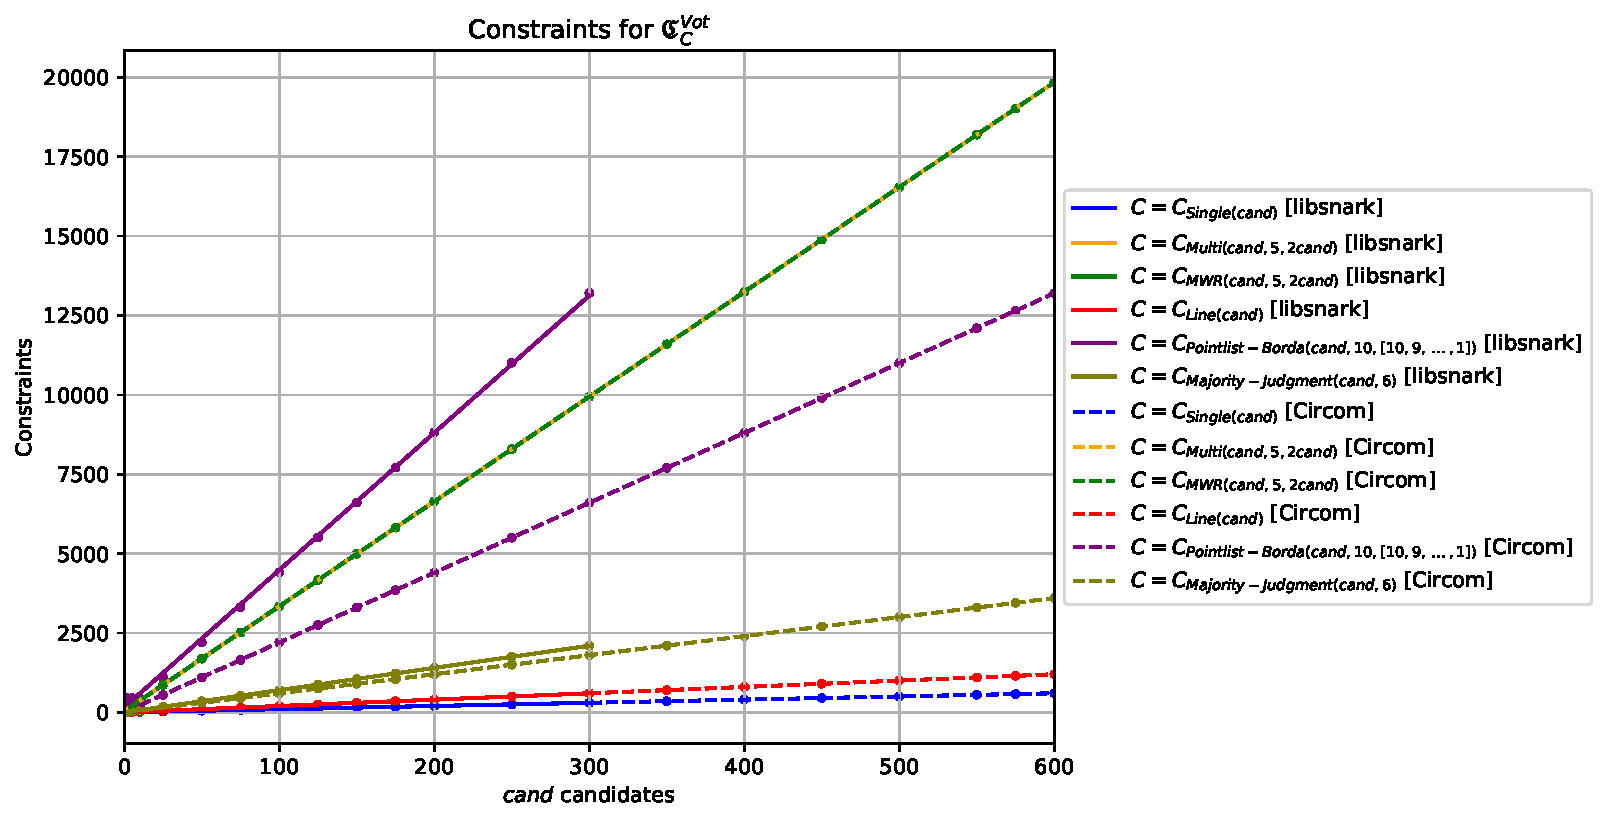
\includegraphics[scale=.6]{../src/benchmarks/plotting/plots/voting/Comparison/linear/VotingComparisonLinearConstraints.pdf}
        \caption{Number of constraints.}
        \label{fig:plots:Circom_libsnark_Vot_Linear_Constraints}
    \end{subfigure}
    \\
    \begin{subfigure}{\textwidth}
        \centering
        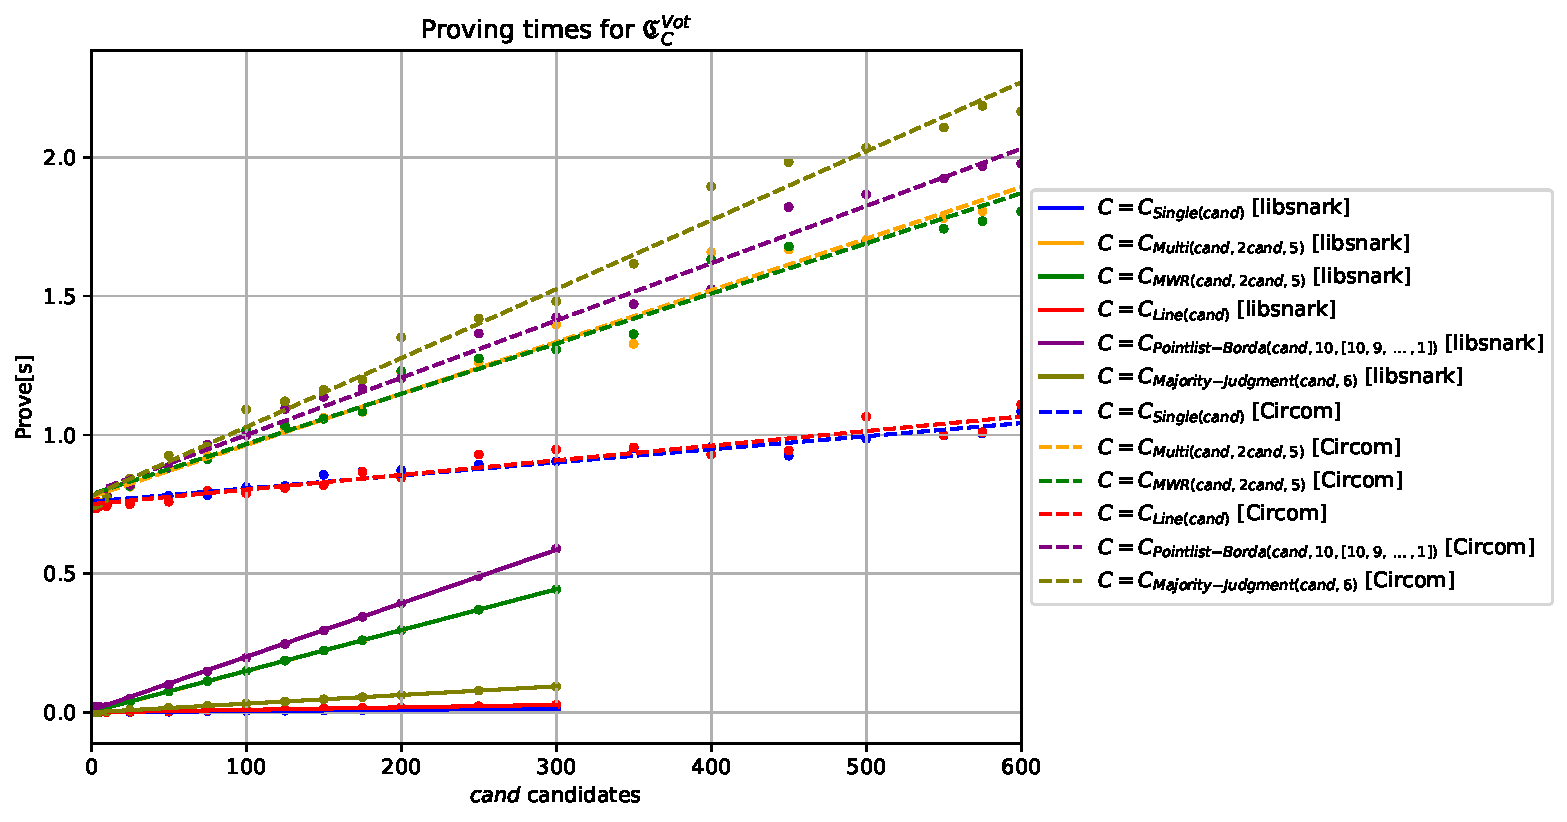
\includegraphics[scale=.6]{../src/benchmarks/plotting/plots/voting/Comparison/linear/VotingComparisonLinearProve[s].pdf}
        \caption{Proving times.}
        \label{fig:plots:Circom_libsnark_Vot_Linear_Prove}
    \end{subfigure}
\end{figure}

\begin{figure}[h]\ContinuedFloat
    \centering
    \begin{subfigure}{\textwidth}
        \centering
        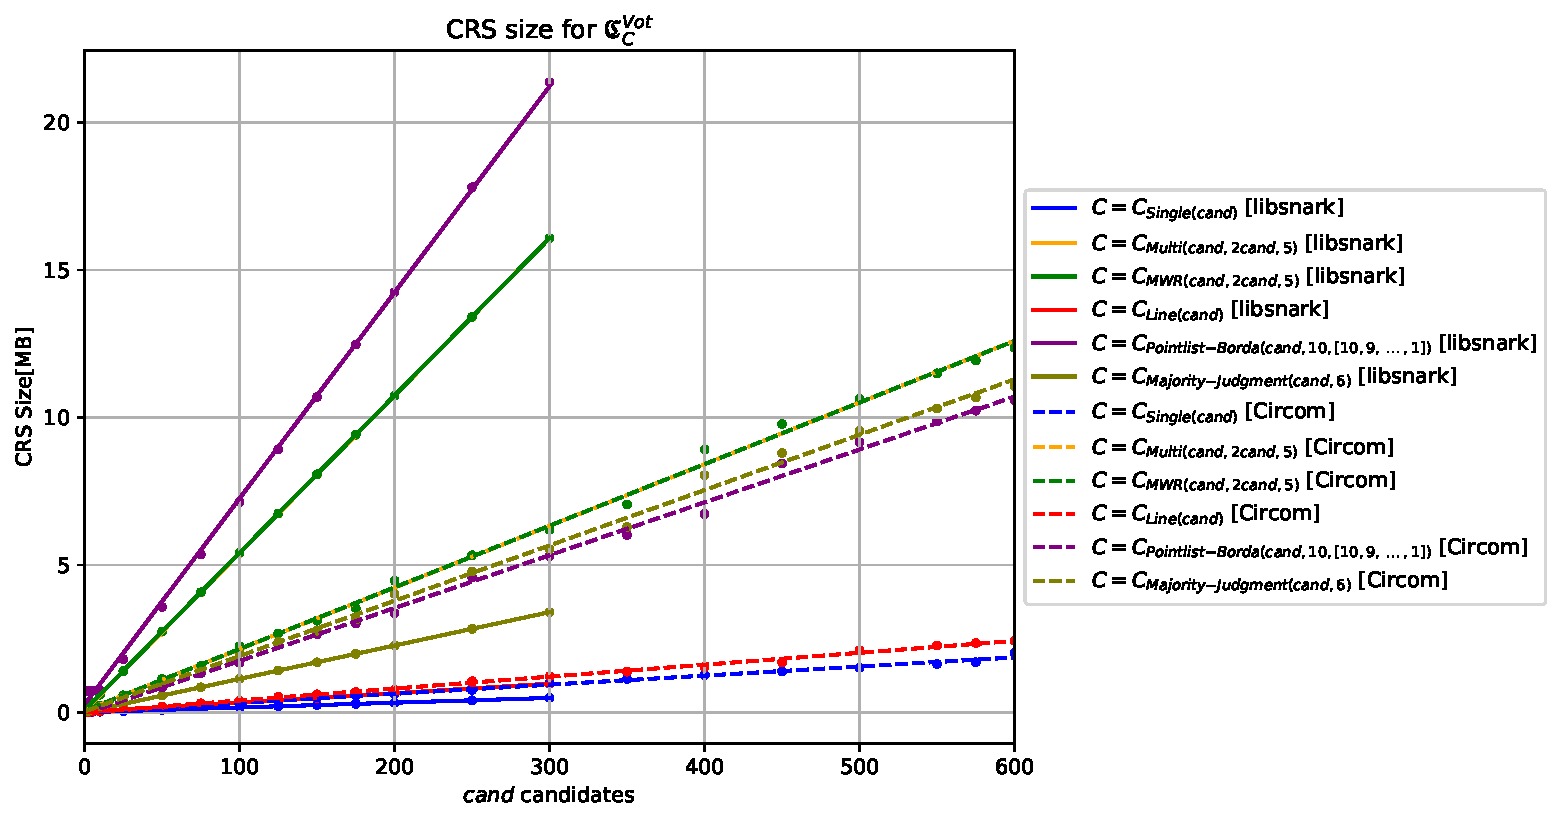
\includegraphics[scale=.6]{../src/benchmarks/plotting/plots/voting/Comparison/linear/VotingComparisonLinearCRS Size[MB].pdf}
        \caption{Size of the $CRS$.}
        \label{fig:plots:Circom_libsnark_Vot_Linear_CRSSize}
    \end{subfigure}
    \\
    \begin{subfigure}{\textwidth}
        \centering
        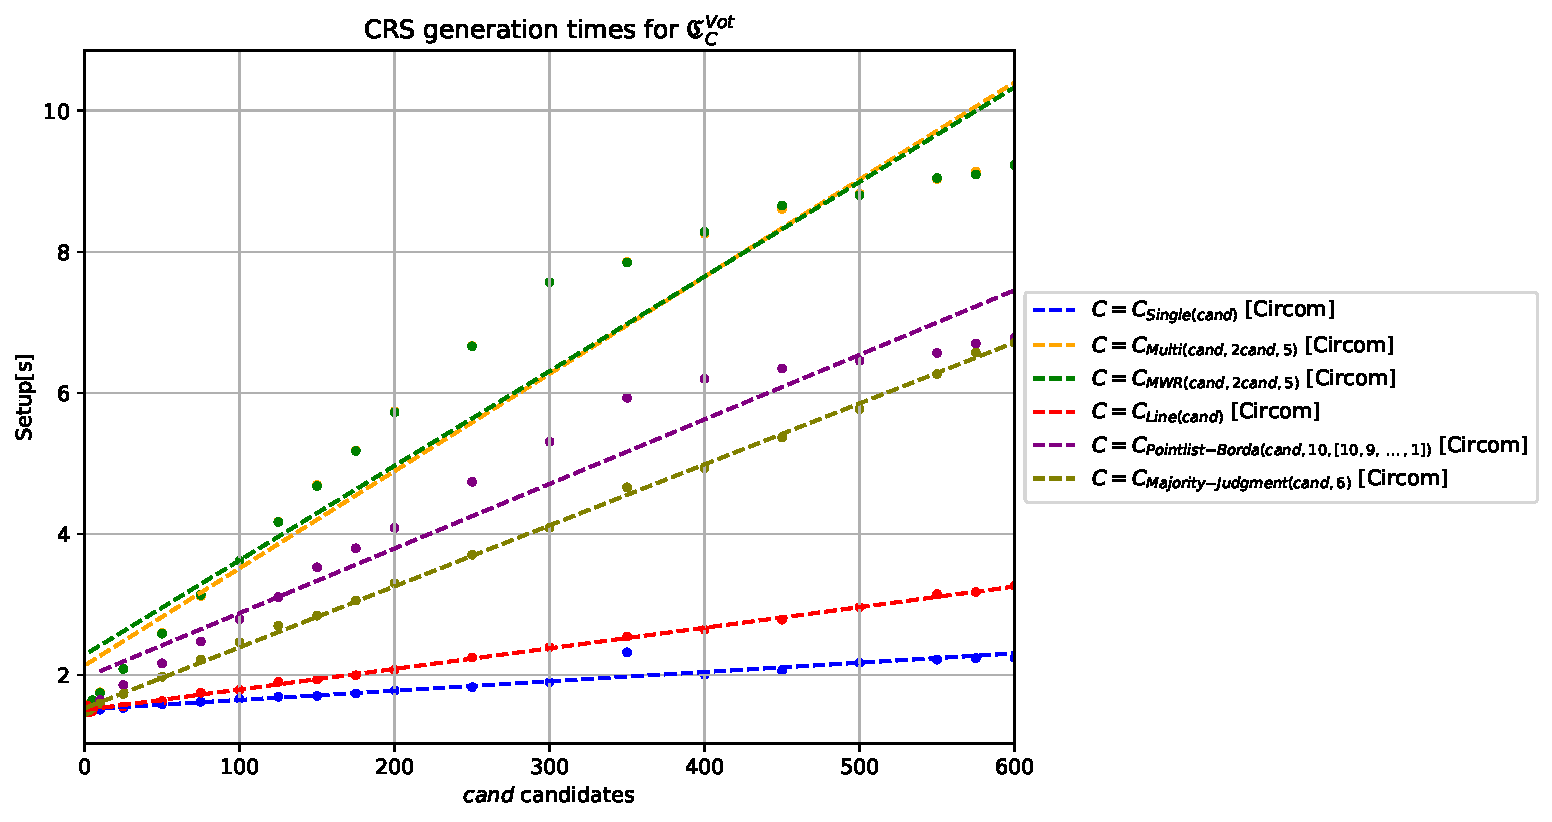
\includegraphics[scale=.6]{../src/benchmarks/plotting/plots/voting/Comparison/linear/VotingComparisonLinearSetup[s].pdf}
        \caption{Time needed to generate the $CRS$ from an existing \UseVerb{ptau} file.\cref{footnote:noCompForCRSGenerationTimes}}
        \label{fig:plots:Circom_libsnark_Vot_Linear_Setup}
    \end{subfigure}
    \caption{Number of constraints, proving times, $CRS$ sizes and $CRS$ generation times needed for the \gls{g16snark} over for $\mathfrak{C}_{C}^{Vot}$ in Circom and in libsnark, where $C$ is a choice space for which the contraint count of $\mathfrak{C}_C^{Vot}$ scales linearly with the candidate count.}
    \label{fig:plots:Circom_libsnark_Vot_Linear}
\end{figure}

\begin{figure}[h]
    \centering
    \begin{subfigure}{\textwidth}
        \centering
        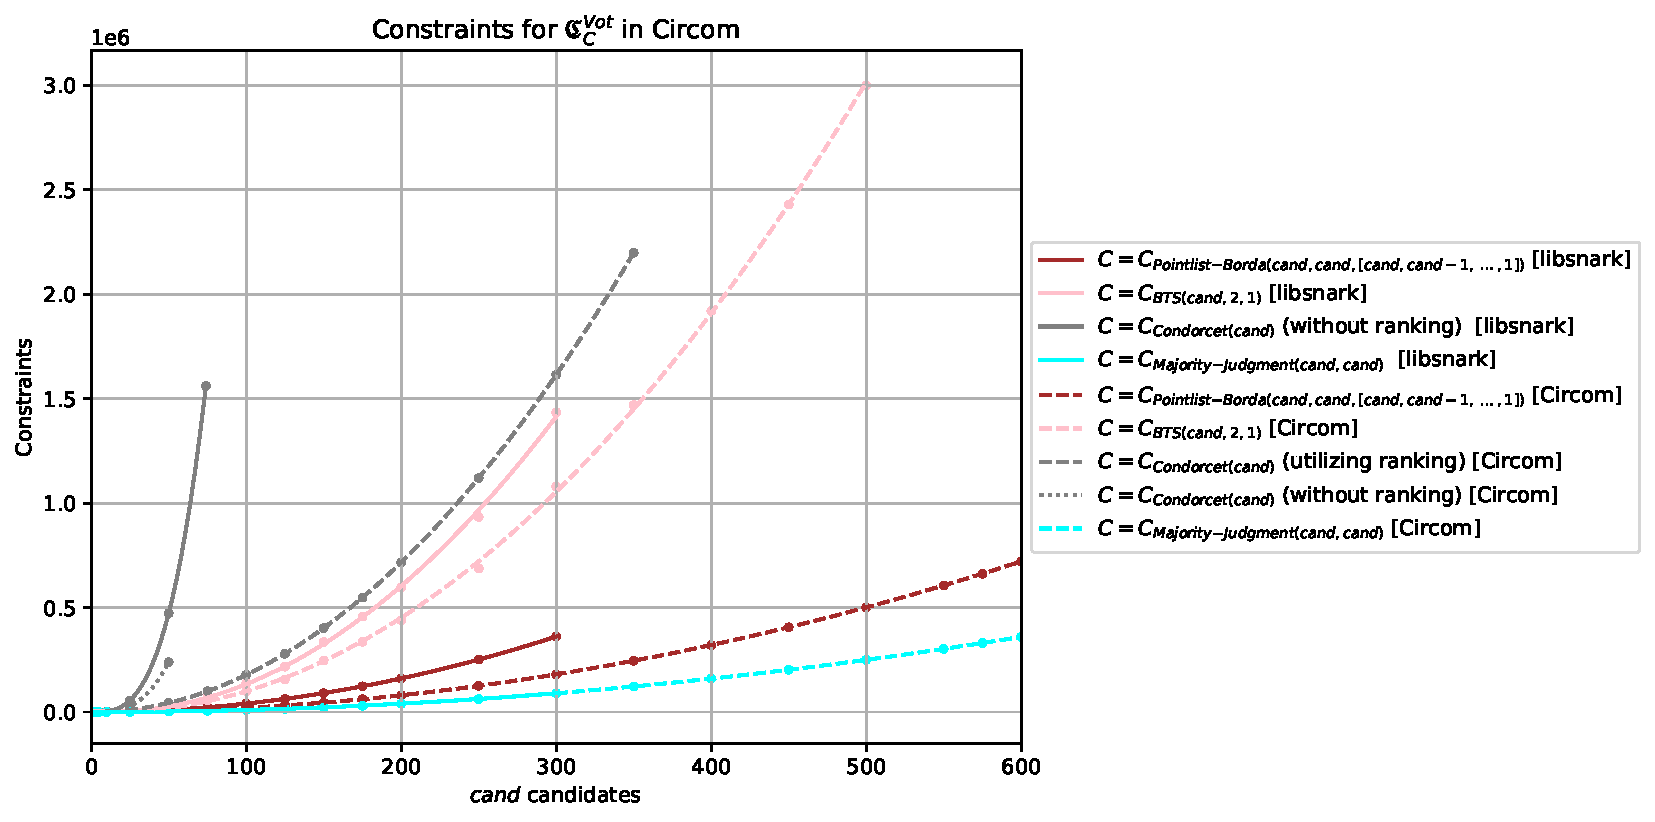
\includegraphics[scale=.6]{../src/benchmarks/plotting/plots/voting/Comparison/quadratic/VotingComparisonQuadraticConstraints.pdf}
        \caption{Number of constraints.}
        \label{fig:plots:Circom_libsnark_Vot_Quadratic_Constraints}
    \end{subfigure}
    \\
    \begin{subfigure}{\textwidth}
        \centering
        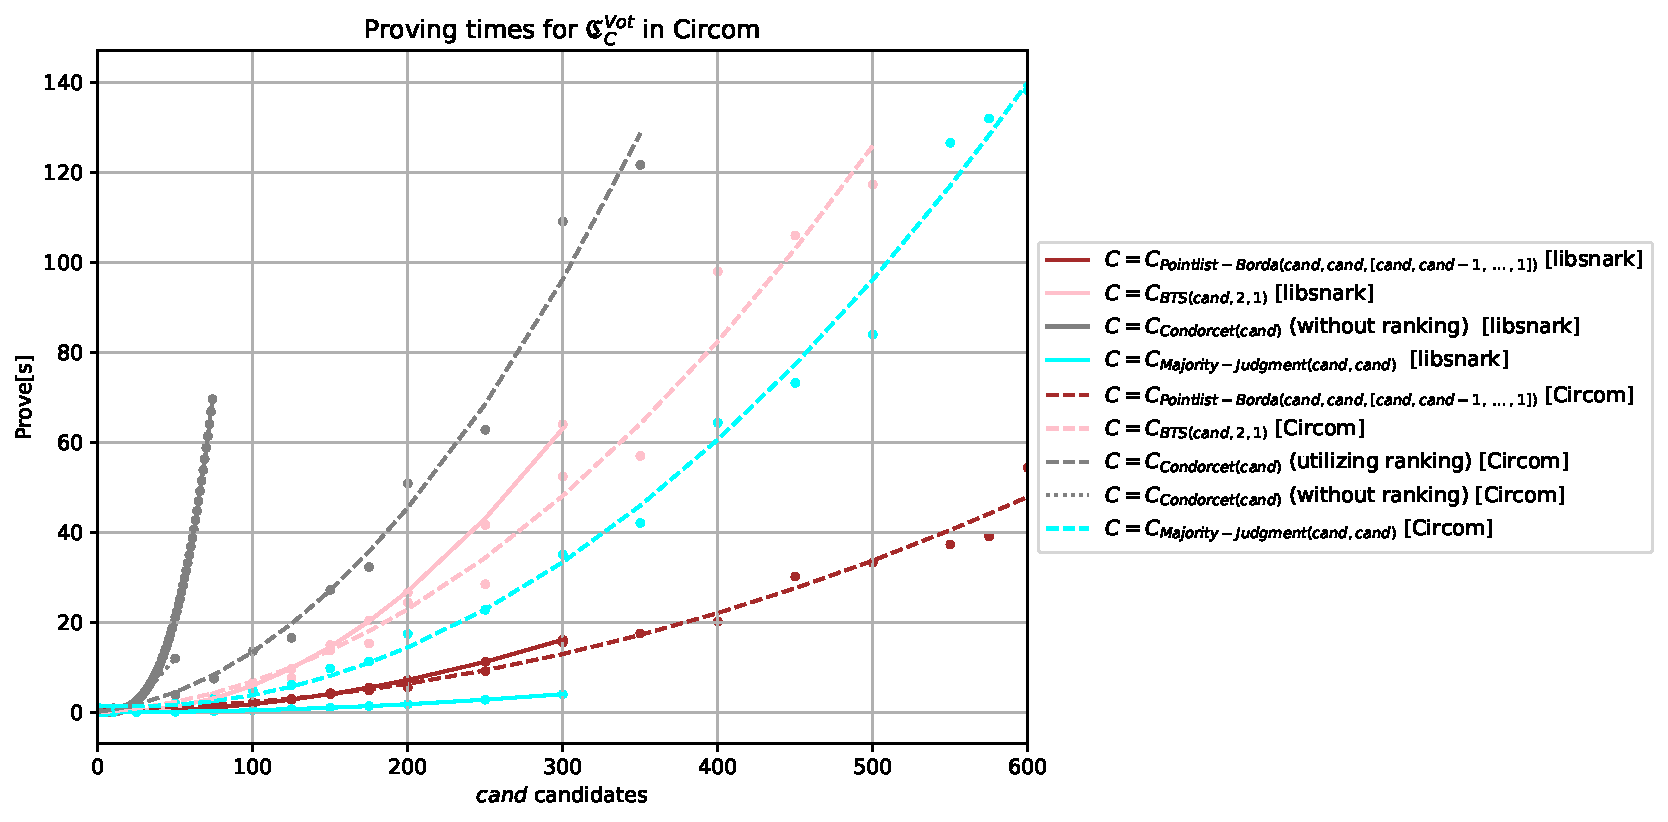
\includegraphics[scale=.6]{../src/benchmarks/plotting/plots/voting/Comparison/quadratic/VotingComparisonQuadraticProve[s].pdf}
        \caption{Proving times.}
        \label{fig:plots:Circom_libsnark_Vot_Quadratic_Prove}
    \end{subfigure}
\end{figure}

\begin{figure}[h]\ContinuedFloat
    \centering
    \begin{subfigure}{\textwidth}
        \centering
        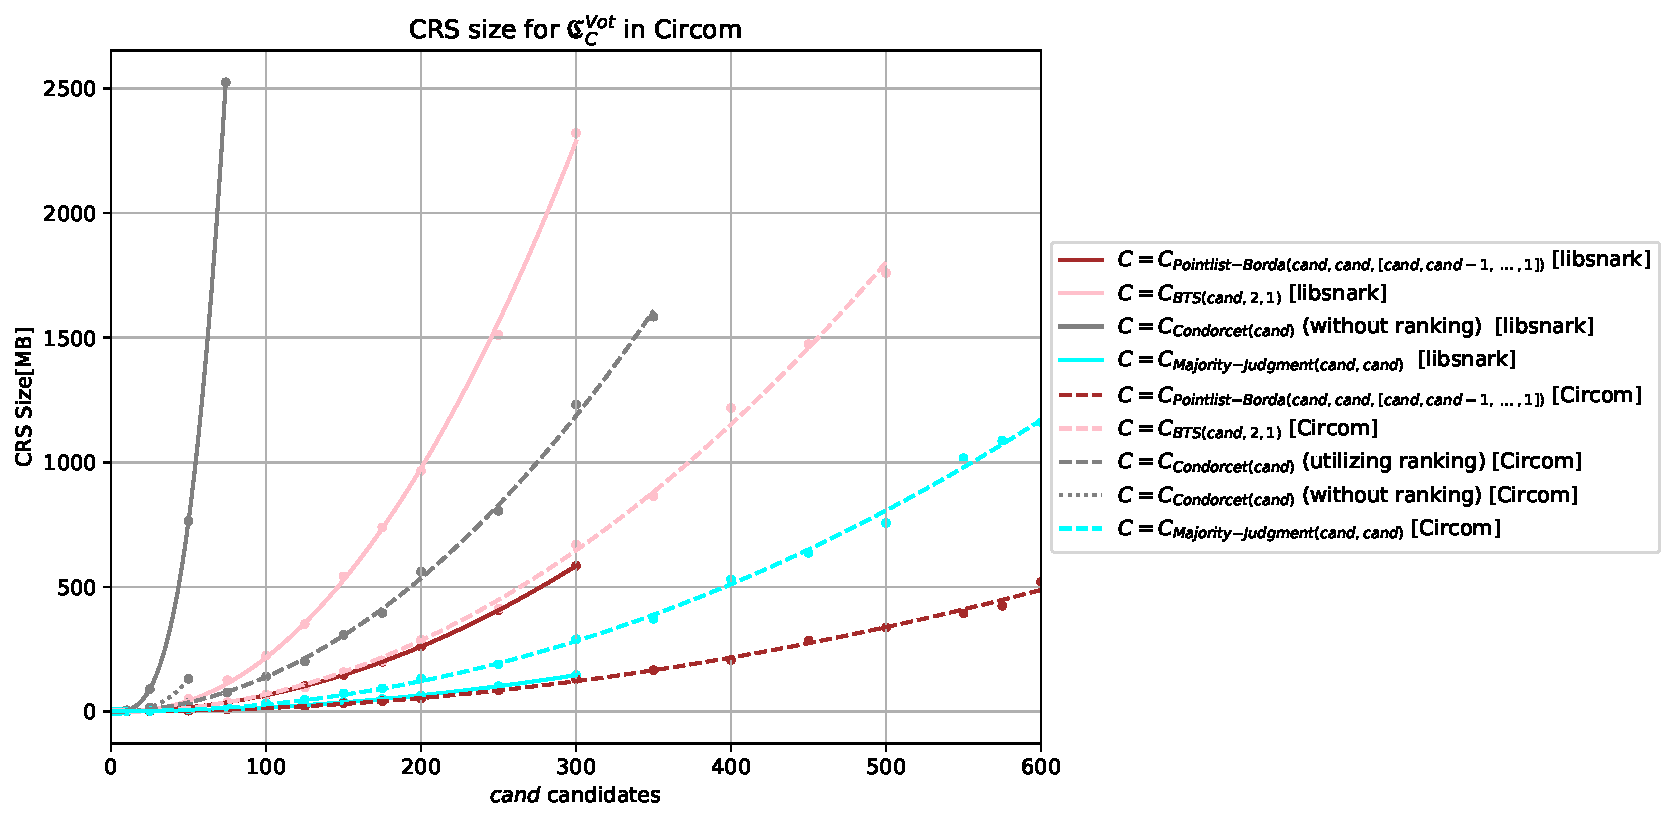
\includegraphics[scale=.6]{../src/benchmarks/plotting/plots/voting/Comparison/quadratic/VotingComparisonQuadraticCRS Size[MB].pdf}
        \caption{Size of the $CRS$.}
        \label{fig:plots:Circom_libsnark_Vot_Quadratic_CRSSize}
    \end{subfigure}
    \\
    \begin{subfigure}{\textwidth}
        \centering
        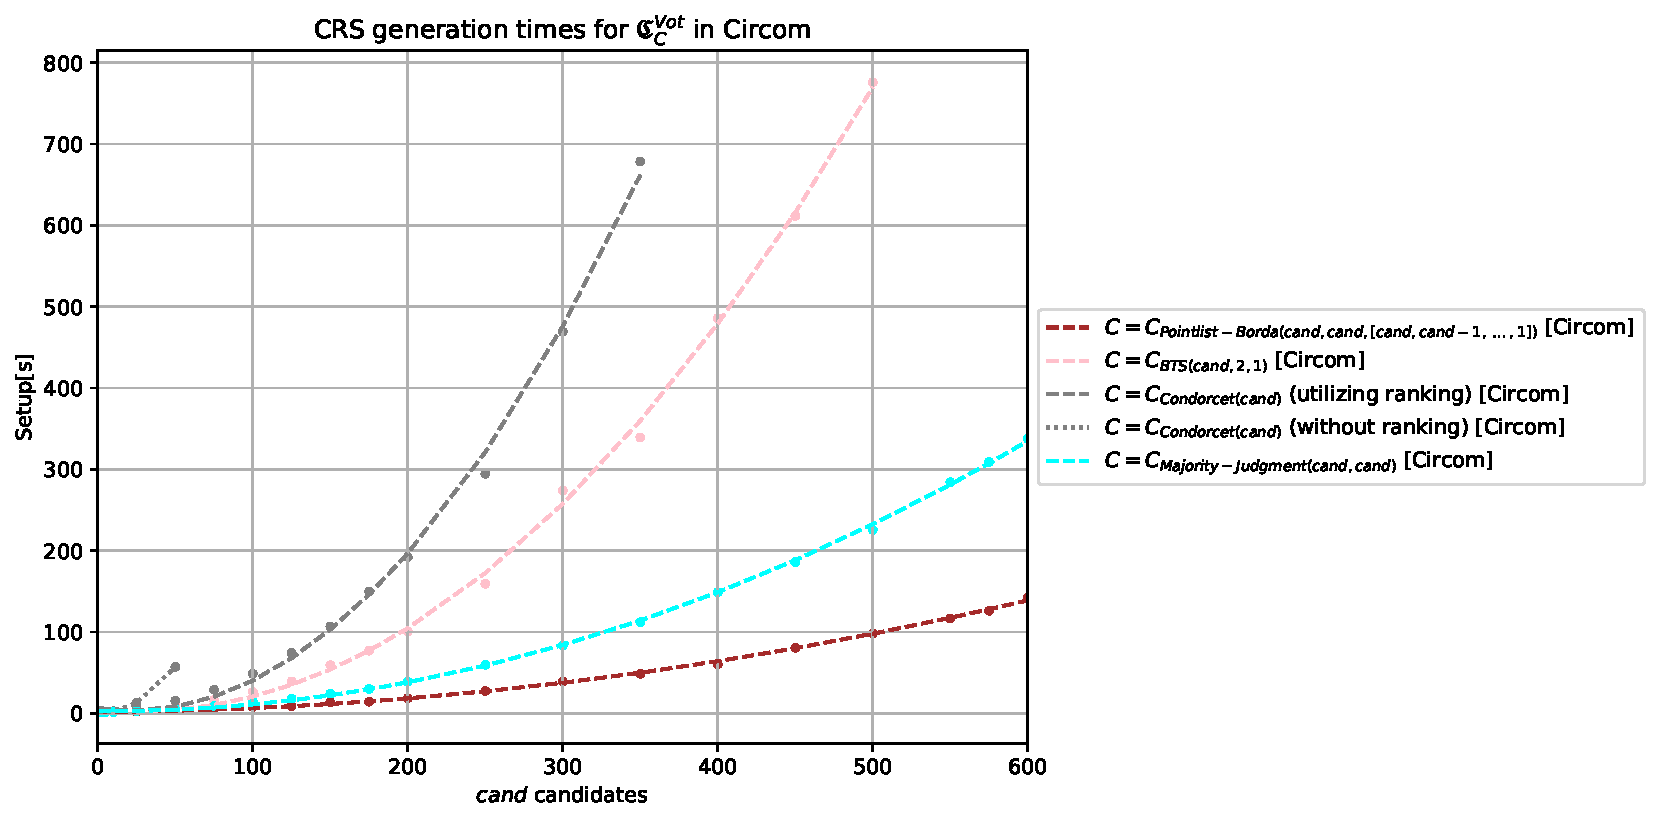
\includegraphics[scale=.6]{../src/benchmarks/plotting/plots/voting/Comparison/quadratic/VotingComparisonQuadraticSetup[s].pdf}
        \caption{Time needed to generate the $CRS$ from an existing \UseVerb{ptau} file.\cref{footnote:noCompForCRSGenerationTimes}}
        \label{fig:plots:Circom_libsnark_Vot_Quadratic_Setup}
    \end{subfigure}
    \caption{Number of constraints, proving times, $CRS$ sizes and $CRS$ generation times needed for the \gls{g16snark} over for $\mathfrak{C}_{C}^{Vot}$ in Circom and in libsnark, where $C$ is a choice space for which the contraint count of $\mathfrak{C}_C^{Vot}$ scales quadratically with the candidate count.}
    \label{fig:plots:Circom_libsnark_Vot_Quadratic}
\end{figure}

\todo{Discussion}

\section{Asserting Ballot Validity via $\mathfrak{C}_C^{Ballot\text{-}Validity}$}
\label{section:results:assertCombined}
The circuit $\mathfrak{C}_C^{Ballot\text{-}Validity}$ combines $\mathfrak{C}_C^{Enc}$ and $\mathfrak{C}_C^{Vot}$ for complete proofs of ballot validity \cref{section:ourVotingSchemes:ballotValidity}.
As in \cref{section:results:assertEncryption}, we use either a Montgomery Curve or the isomorphic Twisted Edwards curve for the encryption part.

The results of our benchmarks and the comparison with the results obtained by Huber et. al. are shown in Figures \ref{fig:plots:Combined_Single}, \ref{fig:plots:Combined_Multi}, \ref{fig:plots:Combined_Borda}, \ref{fig:plots:Combined_Condorcet} and \ref{fig:plots:Combined_MajorityJudgment}.
Here, we show our results seperately for every election type or family of election types to limit the amount of data presented in each plot.
Additionally, we only show the candidate count here and omit the results for proving times, $CRS$ sizes and $CRS$ generation times.
These metrics depend directly on the candidate count and the connection beteeen them has been explored in \cref{section:results:assertEncryption} and \cref{section:results:asertVoting} in detail.
However, the remaining results are also presented in \cref{todo}. \todo{Make in Appendix}

\begin{figure}[h]
    \centering
    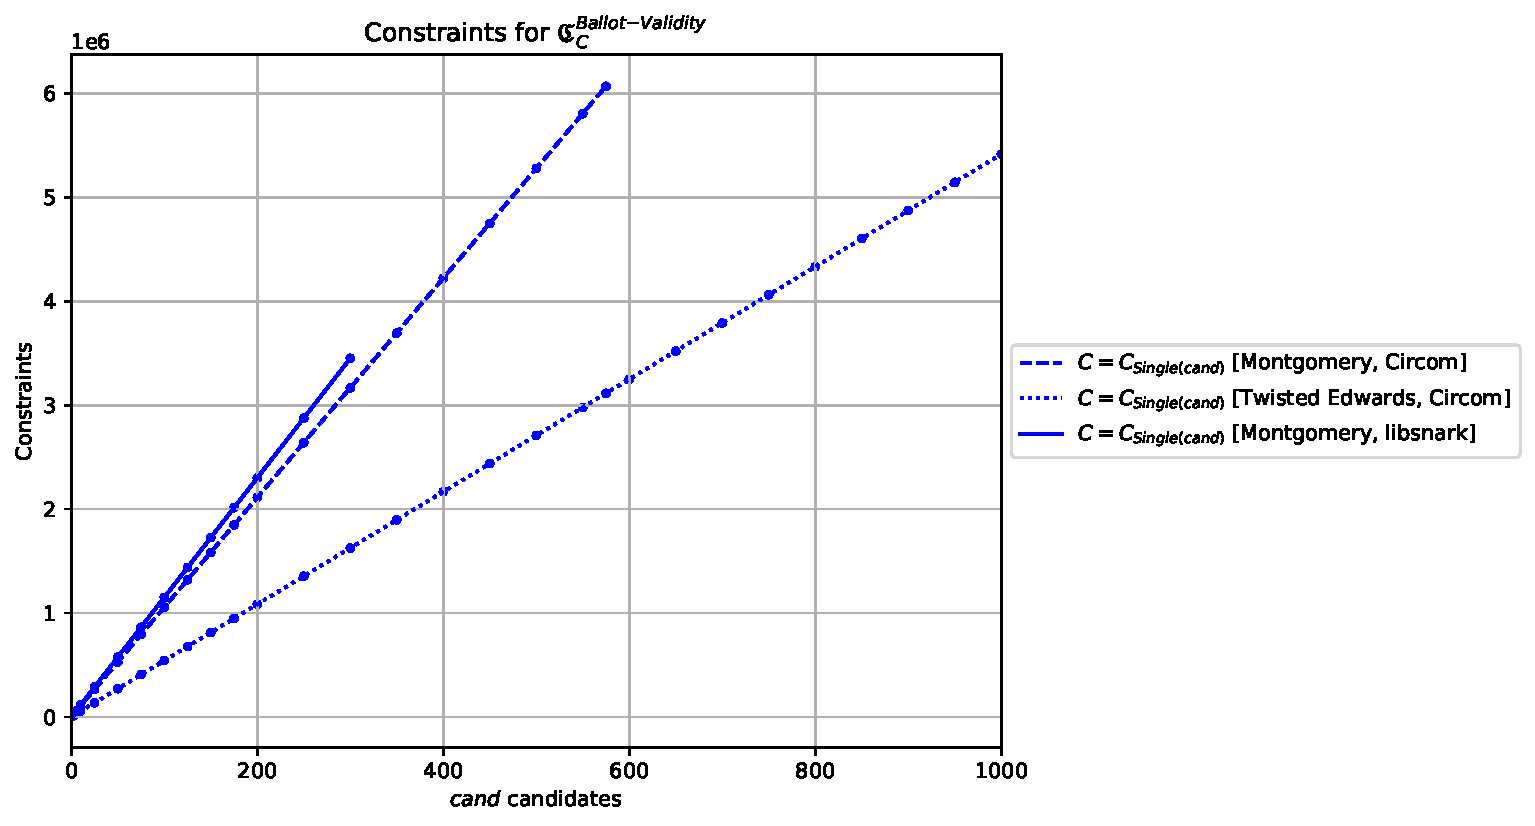
\includegraphics[scale=.6]{../src/benchmarks/plotting/plots/combined/Comparison/Single/CombinedComparisonSingleConstraints.pdf}
    \caption{Number of constraints needed for the \gls{g16snark} over for $\mathfrak{C}_{C_{Single(cand)}}^{Ballot\text{-}Validity}$ in Circom and in libsnark.}
    \label{fig:plots:Combined_Single}
\end{figure}
\begin{figure}[h]
    \centering
    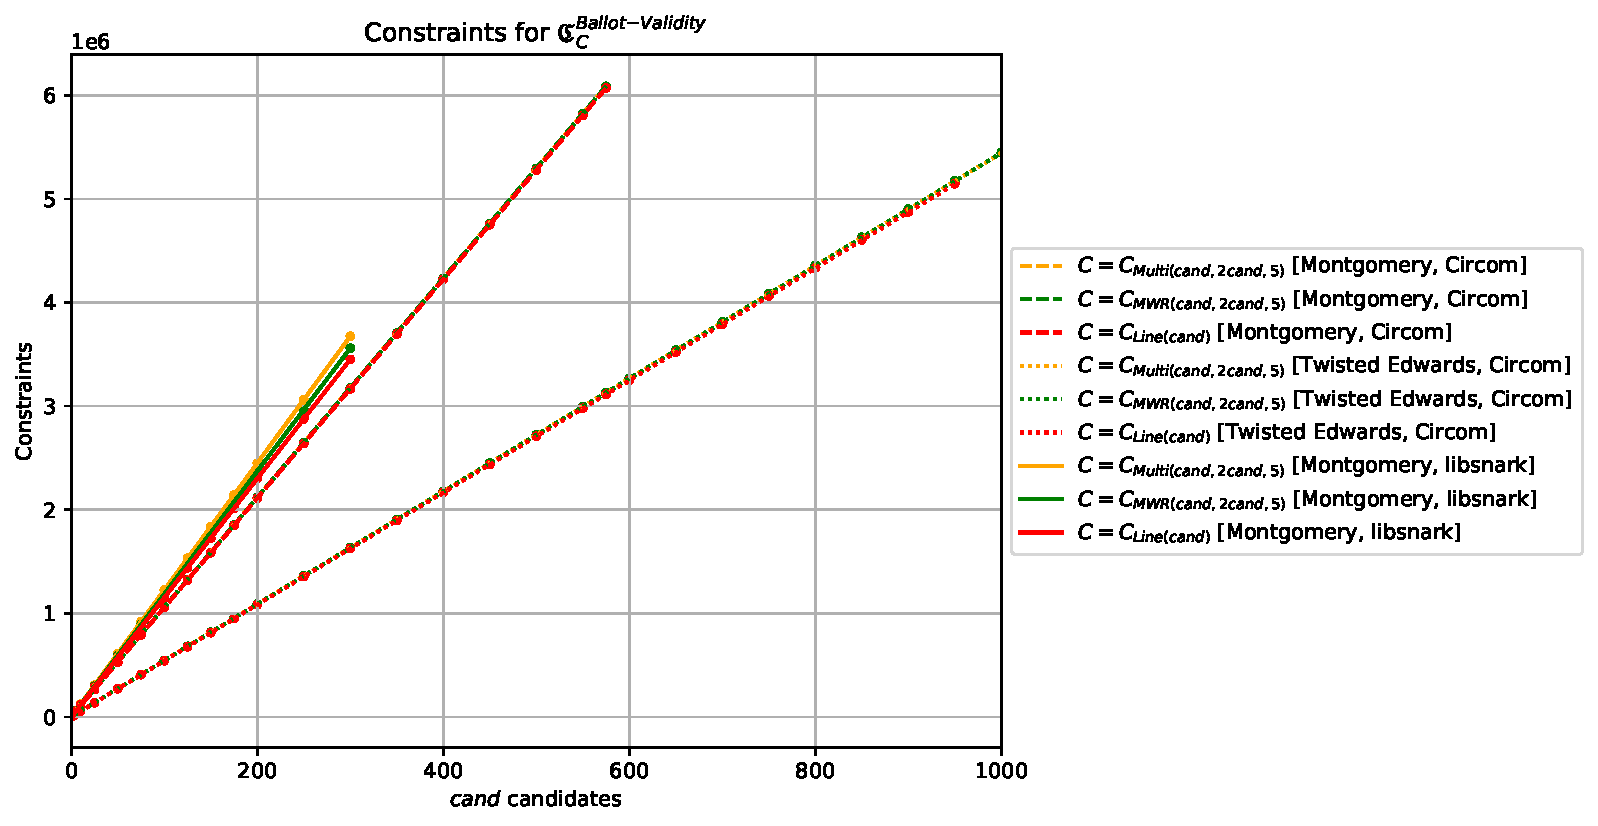
\includegraphics[scale=.6]{../src/benchmarks/plotting/plots/combined/Comparison/Multi/CombinedComparisonMultiConstraints.pdf}
    \caption{Number of constraints needed for the \gls{g16snark} over for $\mathfrak{C}_{C}^{Ballot\text{-}Validity}$ in Circom and in libsnark, where $C\in\{C_{Multi(cand, 2cand, 5)}, C_{Line(cand)}, C_{MWR(cand, 2cand, 5)}\}$}
    \label{fig:plots:Combined_Multi}
\end{figure}
\begin{figure}[h]
    \centering
    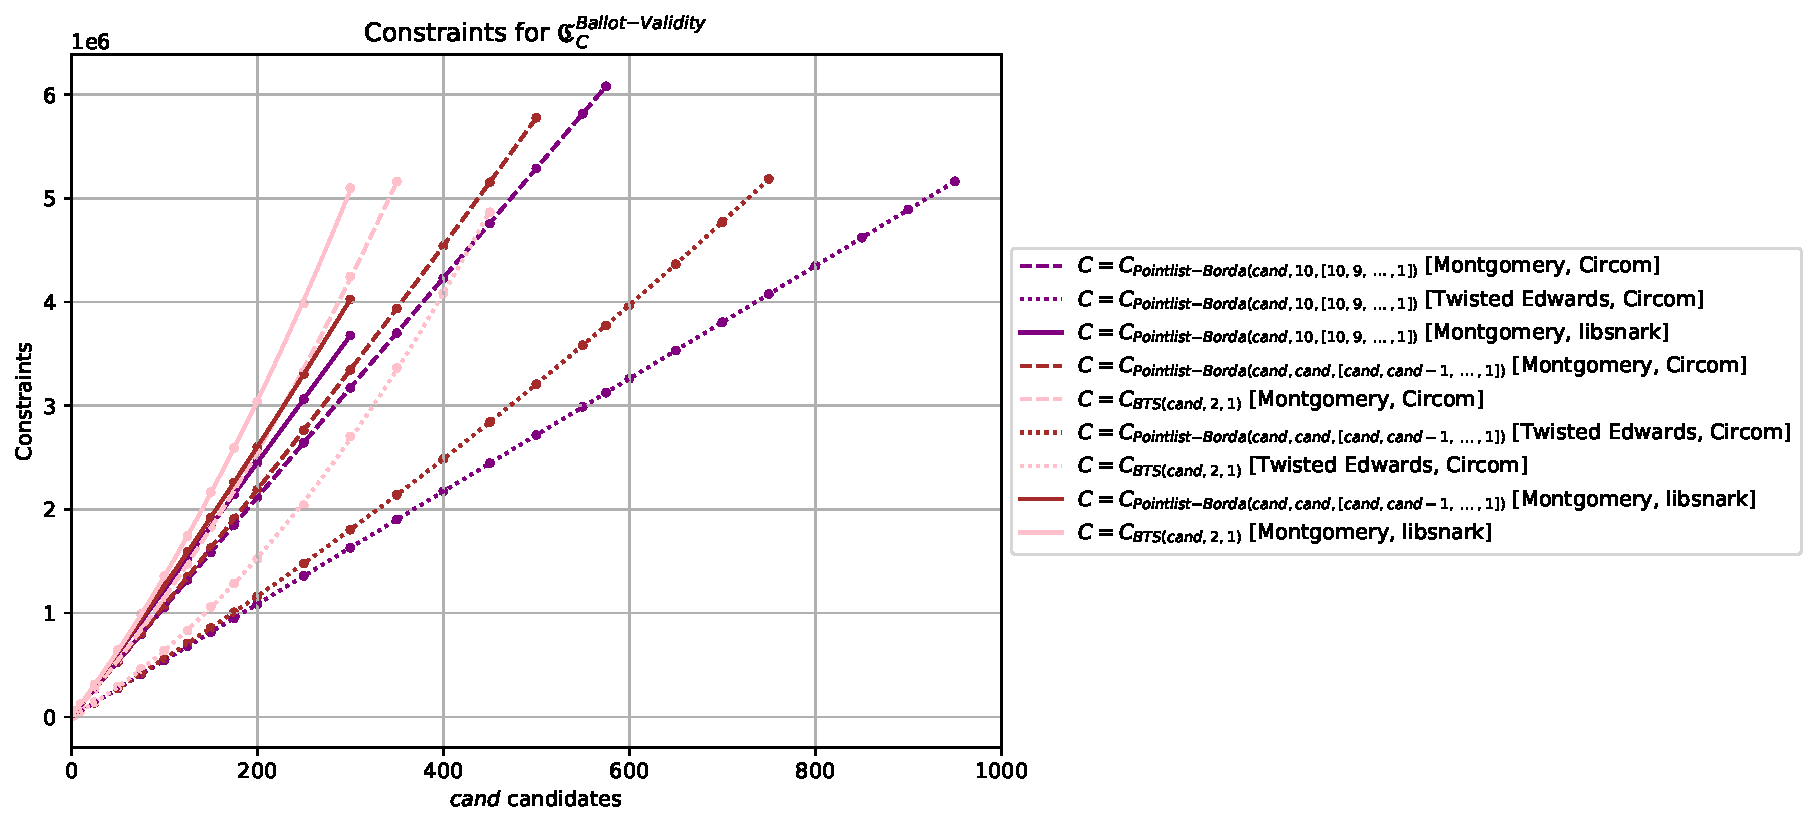
\includegraphics[scale=.6]{../src/benchmarks/plotting/plots/combined/Comparison/Borda/CombinedComparisonBordaConstraints.pdf}
    \caption{Number of constraints needed for the \gls{g16snark} over for $\mathfrak{C}_{C}^{Ballot\text{-}Validity}$ in Circom and in libsnark, where $C\in\{C_{Pointlist\text{-}Borda(cand, 10, [10,9,\dots, 1])}, C_{Pointlist\text{-}Borda(cand, cand, [cand, cand-1, \dots, 1])}, C_{BTS(cand, 2, 1)}\}$}
    \label{fig:plots:Combined_Borda}
\end{figure}
\begin{figure}[h]
    \centering
    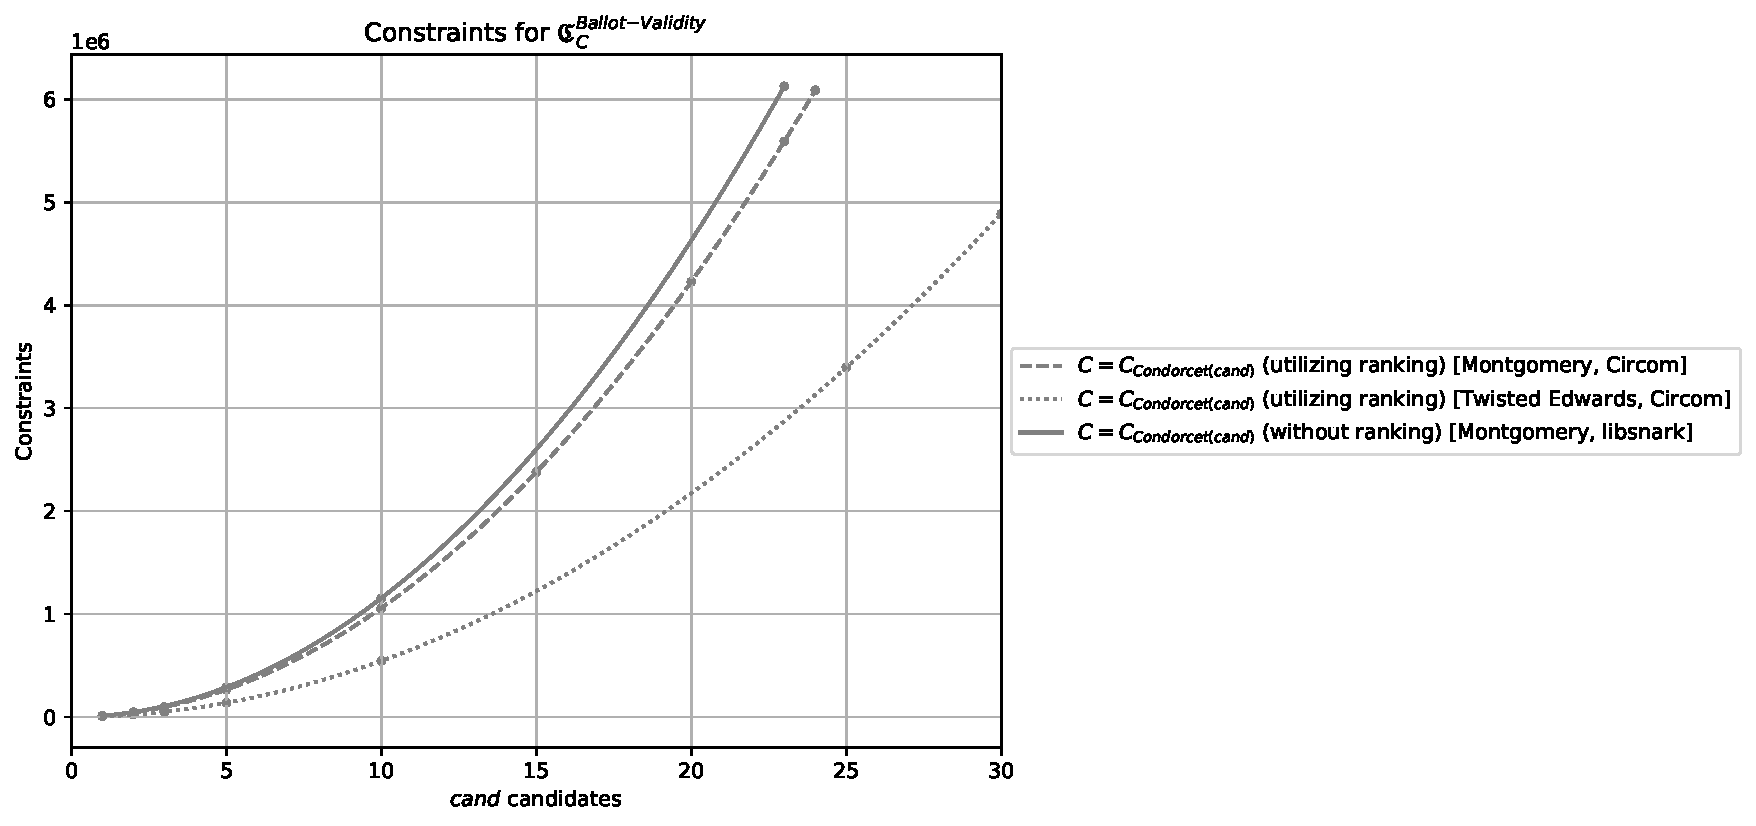
\includegraphics[scale=.6]{../src/benchmarks/plotting/plots/combined/Comparison/Condorcet/CombinedComparisonCondorcetConstraints.pdf}
    \caption{Number of constraints needed for the \gls{g16snark} over for $\mathfrak{C}_{C_{Condorcet(cand)}}^{Ballot\text{-}Validity}$ in Circom and in libsnark.}
    \label{fig:plots:Combined_Condorcet}
\end{figure}
\begin{figure}[h]
    \centering
    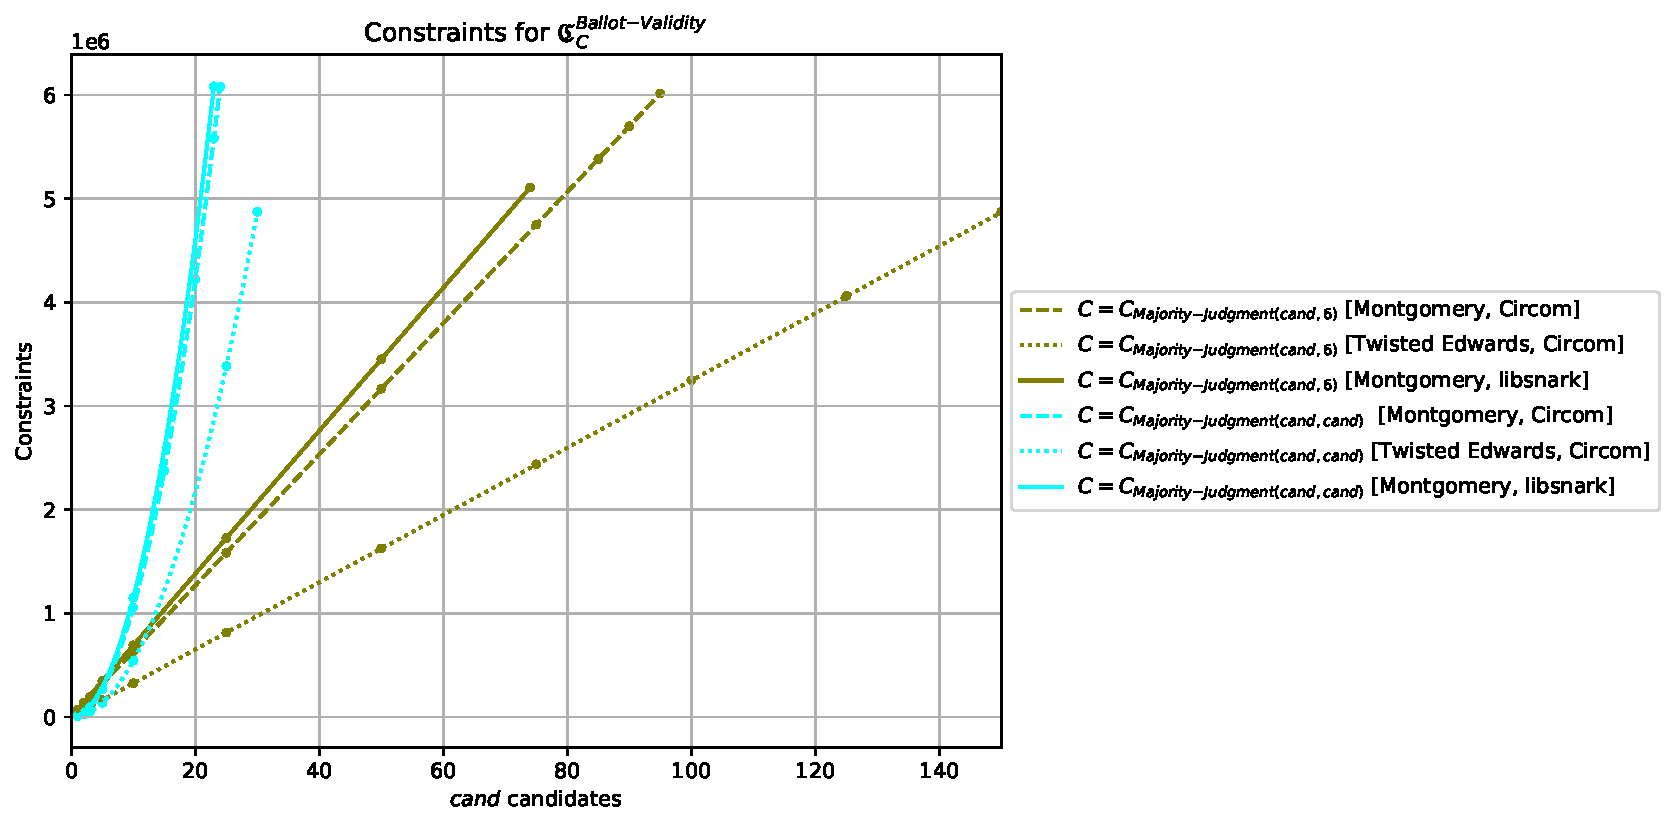
\includegraphics[scale=.6]{../src/benchmarks/plotting/plots/combined/Comparison/MajorityJudgment/CombinedComparisonMajorityJudgmentConstraints.pdf}
    \caption{Number of constraints needed for the \gls{g16snark} over for $\mathfrak{C}_{C}^{Ballot\text{-}Validity}$ in Circom and in libsnark, where $C\in\{C_{Majority\text{-}Judgment(cand, 6)}, C_{Majority\text{-}Judgment(cand, cand)}\}$}
    \label{fig:plots:Combined_MajorityJudgment}
\end{figure}

% into the results for voting schemes where the number of entries in a ballot scales linearly with the candidate count and the results for voting schemes where the number of entries in a ballot scales quadratically with the candidate count.

% Additionally, we compare our results to those obtained by Huber et. al. as shown in \cref{fig:benchmarks:combinedComp}.

\todo{Discussion}